\documentclass{../../slides-style}

\slidetitle[Введение]{Программирование на Java}{19.09.2026}

\begin{document}

    \begin{frame}[plain]
        \titlepage
        \begin{textblock}{3}(4.5,-0.5)
            
\includegraphics[width=\textwidth]{javaLogo.png}
        \end{textblock}
    \end{frame}

    \section{Введение}

    \begin{frame}{Формальности}
        \begin{outline}
            \1 Практический курс, в формате мастер-классов и командной работы на паре
            \1 Будет несколько домашних заданий, две \enquote{контрольные} и пара с докладами
                \2 По домашним работам будут дедлайны, -1 балл за каждую неделю просрочки, начиная с нулевой
                \2 Контрольные в форме устной беседы
                \2 Баллы за домашние и контрольные приводятся к диапазону 0-100, берётся \emph{минимум}
                \2 К нему прибавляются баллы за работу в аудитории и за доклады
            \1 Условия, материалы и сдача домашек через \url{https://hwproj.ru/courses/50105}
            \1 Среда программирования --- какая угодно
                \2 OpenIDE, GigaIDE, VS Code, IntelliJ IDEA (если сможете её достать)
            \1 Преподаватели: Юрий Литвинов (y.litvinov@spbu.ru), Юрий Уфимцев (YuriUfimtsev@yandex.ru)
        \end{outline}
    \end{frame}

    \begin{frame}{Что будет в курсе}
        \begin{outline}
            \1 Особенности синтаксиса Java
            \1 Модульное тестирование в Java (JUnit, Mockito, Hamcrest)
            \1 Коллекции стандартной библиотеки
            \1 Stream API
            \1 Работа с базами данных (JDBC, JPA, Hibernate, Spring Data JPA)
            \1 Веб-сервисы и веб-приложения, Spring
            \1 Веб-API --- REST, gRPC, GraphQL
            \1 Очереди сообщений, Apache Kafka, RabbitMQ
            \1 Многопоточное программирование --- synchronized, Future, пул потоков
        \end{outline}
    \end{frame}

    \section{Java}

    \begin{frame}{Язык Java}
        \begin{outline}
            \1 Появился в 1995 году, актуальная версия --- Java 27
                \2 Актуальная LTS-версия --- Java 25
                \2 Всё ещё популярна Java 8
            \1 Объектно-ориентированный язык с сильной типизацией
            \1 Прежде всего --- для разработки прикладного программного обеспечения
                \2 Большая часть современного Enterprise --- на Java
            \1 Использует виртуальную машину (compile once --- run everywhere)
            \1 Just-in-time-компиляция с довольно продвинутым рантаймом
            \1 Со всем этим вы должны быть знакомы по Kotlin, потому что он использует инфраструктуру Java
        \end{outline}
        \begin{center}
            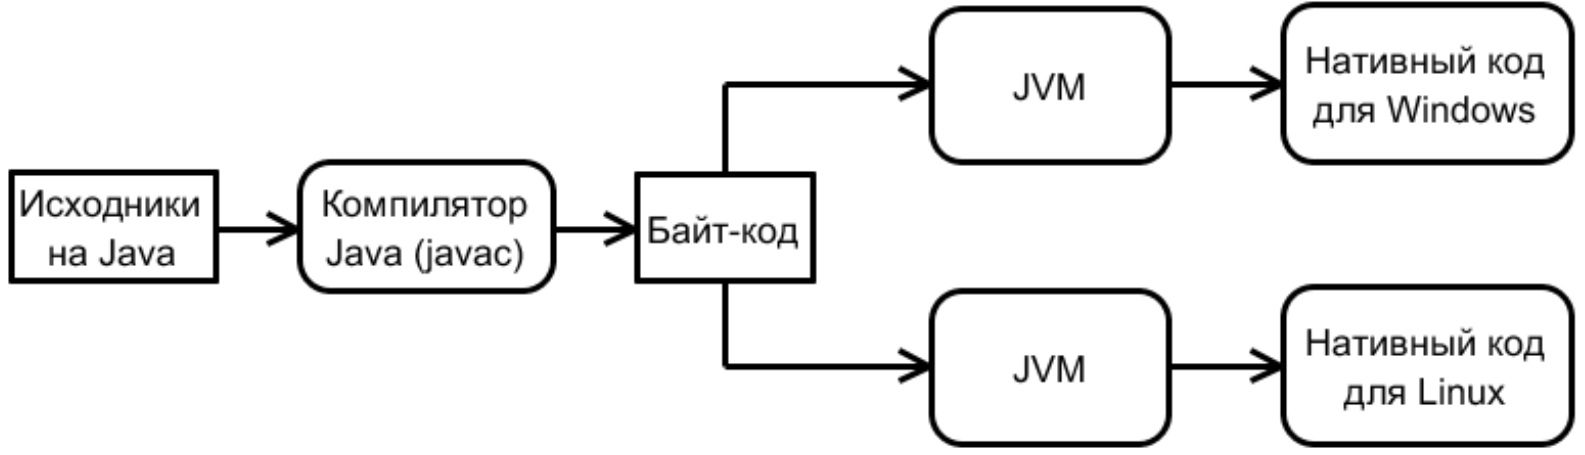
\includegraphics[width=0.7\textwidth]{javaCompiling.png}
        \end{center}
    \end{frame}

    \begin{frame}{Особенности}
        \begin{outline}
            \1 Язык создавался на пике развития ООП, сам сильно повлиял на методологию разработки
                \2 \enquote{Настоящий} теоретически правильный объектно-ориентированный язык
                \2 Создавался на базе опыта C++ с учётом его ошибок (и Smalltalk)
                \2 C\# появился на пять лет позднее и учёл ряд ошибок уже Java
            \1 Практически всё --- объект, иногда даже неожиданно: например, enum-ы --- это полноценные классы с состоянием и методами
            \1 Все методы по умолчанию виртуальные, нет свободных функций
            \1 Много информации о типах известно во время выполнения (развитая рефлексия), расширяемый компилятор
            \1 Несколько странная реализация генериков
            \1 Много разных реализаций виртуальной машины
        \end{outline}
    \end{frame}

    \begin{frame}{Странные аббревиатуры}
        \begin{columns}
            \begin{column}{0.5\textwidth}
                \begin{outline}
                    \1 JVM (Java Virtual Machine) --- то, что исполняет байт-код
                        \2 JIT-компилятор, сборщик мусора и т.п.
                    \1 JRE (Java Runtime Environment) --- среда исполнения (JVM + набор библиотек)
                    \1 JDK (Java Development Kit) --- набор разработчика
                        \2 Компилятор, утилиты для работы с JAR, jshell, javadoc и т.п.
                \end{outline}
            \end{column}
            \begin{column}{0.5\textwidth}
                \begin{center}
                    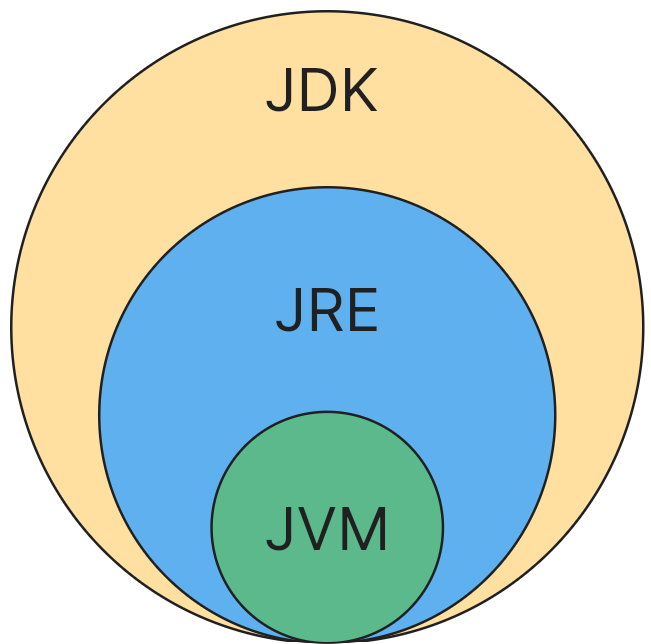
\includegraphics[width=0.7\textwidth]{jvm-jre-jdk.png}
                \end{center}
            \end{column}
        \end{columns}
    \end{frame}

    \begin{frame}{Реализации JDK}
        \begin{columns}
            \begin{column}{0.7\textwidth}
                \begin{outline}
                    \1 OpenJDK --- реализация с открытым исходным кодом от Oracle
                        \2 Что-то вроде референсной реализации, не очень для продуктового окружения
                    \1 Oracle JDK --- официальный JDK от Oracle, платный для коммерческого использования
                    \1 Eclipse Temurin --- бесплатная вендор-нейтральная реализация
                    \1 Azul Zulu --- неплохой коммерческий дистрибутив
                    \1 Axiom JDK, SberJDK --- российские дистрибутивы на базе OpenJDK
                \end{outline}
            \end{column}
            \begin{column}{0.3\textwidth}
                \begin{center}
                    
\includegraphics[width=0.7\textwidth]{openJdkLogo.png}

                    \vspace{5mm}
                    
\includegraphics[width=0.7\textwidth]{oracleJdkLogo.png}

                    \vspace{5mm}
                    
\includegraphics[width=0.7\textwidth]{temurinLogo.png}

                    \vspace{5mm}
                    
\includegraphics[width=0.7\textwidth]{azulLogo.png}

                    \vspace{5mm}
                    
\includegraphics[width=0.7\textwidth]{axiomLogo.png}
                \end{center}
            \end{column}
        \end{columns}
    \end{frame}

    \begin{frame}{Какие ещё языки есть на платформе Java}
        \begin{columns}
            \begin{column}{0.7\textwidth}
                \begin{outline}
                    \1 Kotlin --- \enquote{Java done right}, официальный язык для разработки под Android и неплохой выбор для Enterprise-разработки
                    \1 Scala --- в основном функциональный язык, для сурового бэкенда
                        \2 Не стал суперпопулярен, хотя вовсе не эзотерика --- сложный
                    \1 Groovy --- в основном для мелких скриптов (например, систем сборки)
                    \1 Clojure --- диалект LISP для JVM (функциональный)
                        \2 Скорее эзотерика
                    \1 Многие другие
                \end{outline}
            \end{column}
            \begin{column}{0.3\textwidth}
                \begin{center}
                    
\includegraphics[width=0.7\textwidth]{kotlinLogo.png}

                    \vspace{5mm}
                    
\includegraphics[width=0.7\textwidth]{scalaLogo.png}

                    \vspace{5mm}
                    
\includegraphics[width=0.7\textwidth]{groovyLogo.png}

                    \vspace{5mm}
                    
\includegraphics[width=0.7\textwidth]{clojureLogo.png}
                \end{center}
            \end{column}
        \end{columns}
    \end{frame}

    \section{Типы}

    \begin{frame}{Mandatory slide про стандартные числовые типы}
        \begin{tabu} {| X[0.3 l p] | X[1 l p] | X[0.2 l p] |}
            \tabucline-
            Тип       & Значения                                                                              & Размер  \\
            \tabucline-
            \everyrow{\tabucline-}
            $byte$    & $-2^7..2^7-1 (-128..127)$                                                             & 8 бит   \\
            $short$   & $-2^{15}..2^{15}-1 (-32768..32767)$                                                   & 16 бит  \\
            $int$     & $-2^{31}..2^{31}-1$                                                                   & 32 бит  \\
            $long$    & $-2^{63} .. 2^{63}-1$                                                                 & 64 бит  \\
            $float$   & $-3.4028235E+38..-1.4E-45$ \newline и $1.4E-45..3.4028235E+38$                        & 32 бит  \\
            $double$  & $-1.7976931348623157E+308..-4.9E-324$ \newline и $4.9E-324..1.7976931348623157E+308$  & 64 бит  \\
        \end{tabu}
    \end{frame}

    \begin{frame}{Ссылочные типы и типы-значения}
        \begin{outline}
            \1 Примитивные типы: \mintinline{java}|byte, short, int, long, float, double, boolean, char|
            \1 Ссылочные типы: массивы, классы (в том числе строки и типы-обёртки), интерфейсы, перечисления, аннотации
            \1 Ссылочные типы всегда\footnote{\scriptsize Не совсем всегда, компилятор умеет сам иногда размещать объекты на стеке, если это не ломает семантику} хранятся на куче и передаются по ссылке (точнее, ссылка передаётся по значению), примитивные типы всегда хранятся и передаются по значению
            \1 У каждого типа есть значение по умолчанию --- \mintinline{java}|null| для ссылочных типов (в том числе массивов и строк), нули для всех остальных
            \1 Оператор == для ссылочных типов всегда сравнивает их место в памяти\footnote{\scriptsize Технически это не совсем правда, == сравнивает идентичность объектов, с учётом их перемещений в памяти при сборке мусора и т.п.}
                \2 Строки нельзя сравнивать ==, используйте equals
        \end{outline}
    \end{frame}

    \begin{frame}{Типы-обёртки, что?}
        \begin{outline}
            \1 Классы, соответствующие примитивным типам и поддержанные компилятором
            \1 Boxing/Unboxing
            \1 \mintinline{java}|byte| --- \mintinline{java}|Byte|, \mintinline{java}|short| --- \mintinline{java}|Short|, ну вы поняли
            \1 Не всё так просто: \mintinline{java}|char| --- \mintinline{java}|Character|, \mintinline{java}|int| --- \mintinline{java}|Integer|
            \1 Методы: \mintinline{java}|int ololo = Integer.parseInt("239");|
            \1 Известная \enquote{особенность}:
                \2 \mintinline{java}|Integer.valueOf(127) == Integer.valueOf(127)|
                \2 но \mintinline{java}|Integer.valueOf(128) != Integer.valueOf(128)|
        \end{outline}
    \end{frame}

    \section{Инструменты}

    \begin{frame}{OpenIDE, демонстрация}
        \begin{center}
            \huge{Демонстрация}
        \end{center}
    \end{frame}

    \begin{frame}{Что скачать и поставить}
        \begin{outline}
            \1 JDK 27 (\url{https://jdk.java.net/27/})
                \2 Обратите внимание, JRE --- среда времени выполнения, JDK --- среда времени выполнения + инструменты разработки (включая компилятор)
                \2 Очень желательно добавить javac в PATH и прописать переменную окружения JAVA\_HOME
            \1 OpenIDE (\url{https://openide.ru/}) или VS Code
        \end{outline}
    \end{frame}

    \begin{frame}{Что сдавать в домашках}
        \begin{outline}
            \1 Файлы .java
            \1 Папку .idea
                \2 Кроме workspace.xml, usage.statistics.xml, tasks.xml
            \1 Файлы .iml (если есть)
            \1 Ничего больше
        \end{outline}
    \end{frame}

    \begin{frame}{Как собирать из консоли}
        \begin{outline}
            \1 javac
                \2 javac MyClass.java YetAnotherClass.java
                \2 javac -d classes MyClass.java
                \2 javac -classpath classes;library.jar -d classes MyClass.java
            \1 CLASSPATH
                \2 Набор путей, по которым компилятор и Java-машина ищут классы
                \2 Всегда содержит классы из стандартной библиотеки
                \2 По умолчанию --- текущая директория (``.'')
                \2 Задаётся как список директорий или JAR-файлов, через ``;'' в Windows и через ``:'' во всём остальном
                    \3 JAR-файл --- просто заархивированная папка с классами, по сути --- библиотека
            \1 Системы сборки --- Gradle, Maven, ...
        \end{outline}
    \end{frame}

    \begin{frame}{Как запускать из консоли}
        \begin{outline}
            \1 Нет никакого .exe-шника, виртуальной машине передаётся на исполнение файл с байт-кодом класса
                \2 При желании его можно собрать, но надо специально озаботиться
            \1 Оный класс должен иметь метод \mintinline{java}|public static void main(String[] args)|
            \1 java (javaw)
                \2 java MyClass
                \2 java -classpath classes\_dir;library.jar MyClass
                \2 java -jar library\_with\_main\_class.jar
                    \3 не всё так просто, jar-нику нужен манифест
                \2 Имя запускаемого класса должно быть \textbf{полностью квалифицированным}
                    \3 например, \textit{java com.example.MyClass}
                \2 Нелишне посмотреть документацию, есть много полезных ключей командной строки
            \1 Системы сборки сильно облегчают эту боль
        \end{outline}
    \end{frame}

    \begin{frame}{Некоторые тонкости IntelliJ Platform}
        \begin{outline}
            \1 Есть отдельно меню File -> Settings и отдельно File -> Project Structure
                \2 Settings --- это в основном настройки самой среды
                \2 Project Structure --- это настройки проекта
                    \3 Версия языка (есть отдельно версия языка и отдельно версия SDK)
                    \3 Модули --- в какой папке код, в какой тесты, в какой ресурсы; IntelliJ компилит только папки, отмеченные как Sources или Tests
            \1 Справа вверху --- конфигурации запуска. Там можно настроить, например, параметры командной строки
            \1 Знание основных хоткеев сильно ускоряет разработку
        \end{outline}
    \end{frame}

    \section{Стайлгайд}

    \begin{frame}{Стайлгайд}
        \begin{outline}
            \1 \url{https://google.github.io/styleguide/javaguide.html}
            \1 На что обратить внимание:
                \2 camelCase для методов и \enquote{переменных}, CamelCase для типов, КАПС\_ДЛЯ\_КОНСТАНТ
                \2 Правильные имена пакетов (DNS-имя наоборот + собственно имя пакета)
                \2 \enquote{Египетские} фигурные скобки (так же известны, как K \& R)
                \2 Минимально возможная видимость полей, методов и всего-всего
                    \3 Всегда указывайте модификатор видимости
                \2 Комментарии к каждому классу и каждому public-методу
                    \3 JavaDoc
        \end{outline}
    \end{frame}

    \begin{frame}{JavaDoc}
        \begin{outline}
            \1 Стандартная система генерации документации
            \1 В IntelliJ Platform это Tools -> Generate JavaDoc
            \1 \mintinline{java}|/**  */| --- JavaDoc-комментарий
            \1 Сначала общее описание, затем, опционально, уточняющие тэги
            \1 Тэги:
                \2 \mintinline{java}|@param имя описание параметра|
                \2 \mintinline{java}|@return описание возвращаемого значения|
                \2 \mintinline{java}|@exception ИмяКлассаИсключения описание, когда бросается|
                \2 \mintinline{java}|{@inheritDoc}|
                \2 \mintinline{java}|@see|
            \1 Пустые тэги не очень полезны
        \end{outline}
    \end{frame}

\end{document}
